% Chapter 1

\chapter{Introducción general} % Main chapter title

\label{Chapter1} % For referencing the chapter elsewhere, use \ref{Chapter1} 
\label{IntroGeneral}

%----------------------------------------------------------------------------------------

% Define some commands to keep the formatting separated from the content 
\newcommand{\keyword}[1]{\textbf{#1}}
\newcommand{\tabhead}[1]{\textbf{#1}}
\newcommand{\code}[1]{\texttt{#1}}
\newcommand{\file}[1]{\texttt{\bfseries#1}}
\newcommand{\option}[1]{\texttt{\itshape#1}}
\newcommand{\grados}{$^{\circ}$}

%----------------------------------------------------------------------------------------

En este capitulo se explican las causas que dan origen al dispositivo desarrollado y como este encaja en el proyecto de la empresa Skyloom Global. Se hace una breve descripción de un amplificador óptico, del hardware ya existente y por último se presentan los objetivos y alcances determinados durante la planificación de este trabajo.


%----------------------------------------------------------------------------------------
\section{Contexto y motivación}

La creciente demanda de mayores velocidades de transmisión de información en el ámbito aeroespacial, combinada con las limitaciones de la radiofrecuencia, favorecen el surgimiento de nuevas empresas enfocadas en el desarrollo de nuevas tecnologías capaces de superar estas barreras. Tal es el caso de la empresa Skyloom Global, que propone la creación de una red de satélites de órbita baja (LEO) utilizando enlaces ópticos de alta velocidad.

El núcleo de esta idea reside en un satélite geoestacionario (órbita GEO) al cual los satélites en LEO transmiten la información (denominado \textit{uplink}) para luego descargar esta a una estación terrena (denominado \textit{downlink}). De esta forma se obtiene una alta disponibilidad de los datos ya que el satélite en GEO siempre tiene visión de la Tierra. Un diagrama de esta propuesta se muestra en la figura \ref{fig:propSky}.

\begin{figure}[H]
\centering
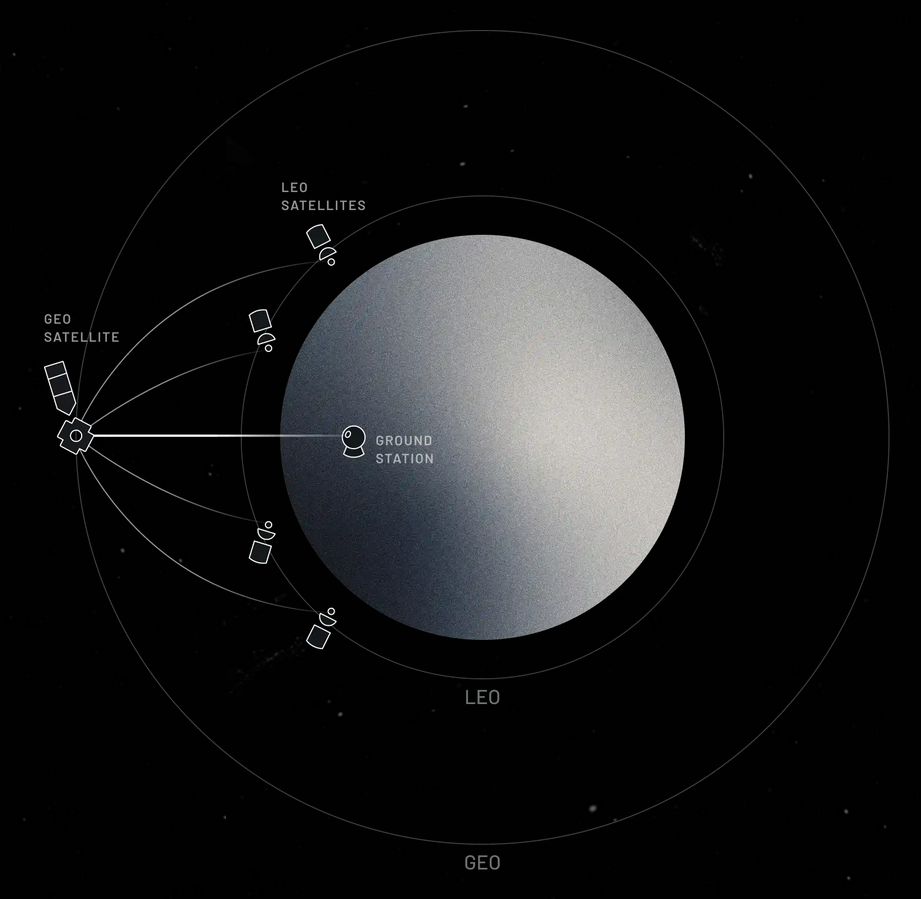
\includegraphics[width=0.85\textwidth]{./Figures/propuesta_skyloom.png}
\caption{Propuesta de la empresa Skyloom Global\protect\footnotemark.}
\label{fig:propSky}
\end{figure}

\footnotetext{Imagen tomada de \url{https://www.skyloom.co/}}

\subsection{Una introducción (no tan corta) a \LaTeX{}}

ABC

\subsubsection{Una subsubsección}

ABCD

%----------------------------------------------------------------------------------------

\section{Producto existente}

asd


%----------------------------------------------------------------------------------------

\section{Objetivos y alcance}

asd

\begin{itemize}
\item Capítulo 1: Introducción general	
\item Capítulo 2: Introducción específica
\item Capítulo 3: Diseño e implementación
\item Capítulo 4: Ensayos y resultados
\item Capítulo 5: Conclusiones
\end{itemize}

sda

\begin{itemize}
\item Capítulo 1: Introducción general	
\item Capítulo 2: Introducción específica
\item Capítulo 3: Diseño e implementación
\item Capítulo 4: Ensayos y resultados
\item Capítulo 5: Conclusiones
\end{itemize}


%----------------------------------------------------------------------------------------

\section{XXX}

asda
 

%----------------------------------------------------------------------------------------
